\documentclass[xcolor=dvipsnames, aspectratio=169]{beamer}
\usepackage[T1]{fontenc}

\usepackage{amsmath, amsfonts, amsthm, amssymb}

\usepackage{fontspec}
\usepackage[mathrm=sym, mathbf=sym]{unicode-math}
\setmainfont{FiraGO}
\setmathfont{Fira Math}
\setmathfont{Latin Modern Math}[range=\mathcal]
\setmathfont{Fira Math}[range=]
\newfontfamily{\firaGo}{FiraGO}

\usepackage{graphicx}
\usepackage{float}
\usepackage{bookmark}
\usepackage{enumitem}
\usepackage{tabularray}

\usepackage{tikz}
\usepackage{pgfplots}
\usetikzlibrary{intersections, angles, calc, positioning}

\definecolor{softyellow}{RGB}{252, 222, 165}
\definecolor{bgg}{HTML}{fafafa}
\definecolor{bbg}{HTML}{23373b}
\definecolor{orang}{HTML}{eb811b}

\usepackage{tcolorbox}
\tcbuselibrary{skins}
\newtcolorbox{marker}[1][]{enhanced,
before skip=2mm,after skip=3mm,
boxrule=0.4pt,left=5mm,right=2mm,top=1mm,bottom=1mm,
colback=yellow!50,
colframe=yellow!20!black,
sharp corners,rounded corners=southeast,arc is angular,arc=3mm,
underlay={%
\path[fill=tcbcolback!80!black] ([yshift=3mm]interior.south east)--++(-0.4,-0.1)--++(0.1,-0.2);
\path[draw=tcbcolframe,shorten <=-0.05mm,shorten >=-0.05mm] ([yshift=3mm]interior.south east)--++(-0.4,-0.1)--++(0.1,-0.2);
\path[fill=yellow!50!black,draw=none] (interior.south west) rectangle node[white]{\huge\bfseries !} ([xshift=4mm]interior.north west);
},
drop fuzzy shadow,#1}

\usepackage{polyglossia}
\setdefaultlanguage{portuguese}
\usepackage{csquotes}
\usepackage[backend=biber, doi=false]{biblatex}
\addbibresource{bibliography.bib}

\newcommand{\bx}{\mathbf{x}}
\newcommand{\bc}{\mathbf{c}}
\newcommand{\bz}{\mathbf{0}}
\newcommand{\bb}{\mathbf{b}}

\title{Epidemia Zumbi \raisebox{-2pt}{
\includegraphics[height=15pt]{zombie-svgrepo-com.pdf}}}
\author{Bruno Sant'Anna\\Jacineide Aquino}
\date{20 de fevereiro de 2024}
\institute{Universidade Federal de Sergipe}

\usetheme[progressbar=foot, block=fill]{metropolis} % https://linorg.usp.br/CTAN/macros/latex/contrib/beamer-contrib/themes/metropolis/doc/metropolistheme.pdf

\setsansfont[BoldFont={Fira Sans SemiBold}]{Fira Sans Book}
\setmonofont{Iosevka Custom Semibold}

\begin{document}
    \metroset{titleformat frame=smallcaps}
    \begin{frame}   
        \maketitle
        \begin{tikzpicture}[remember picture, overlay]
            \node (pic) at ($(current page.east) + (-2.5, 0)$) {
\includegraphics[height=0.6\paperheight]{ufs_vertical_positiva.eps}};
            \filldraw[bgg] (pic.south east) rectangle (pic.north west);
            \node at ($(current page.east) + (-2.5, 0)$) {
\includegraphics[height=0.6\paperheight]{ufs_vertical_positiva.eps}};
        \end{tikzpicture}
    \end{frame}
    \section{Introdução}
    \begin{frame}
        Por meio de equações diferenciais, é possível montar um modelo matématico para entender como uma população varia em um apocalipse zumbi, para isso iremos considerar três grupos
        \begin{itemize}[label=-]
            \item Humanos (H)
            \item Zumbis (Z)
            \item Removidos [mortos que podem retornar como zumbis] (R)
        \end{itemize}
        as funções, $H(t)$, $Z(t)$ e $R(t)$ representam a população de cada grupo em dado instante de tempo.
    \end{frame}
    \begin{frame}
        Nesse modelo também estamos considerando três parametros positivos
        \begin{itemize}[label=-]
            \item $\alpha$ relacionado às interações humano-zumbi que removem zumbis
            \item $\beta$ relacionado às interações humano-zumbi que transformam humanos em zumbis
            \item $\zeta$ relacinado aos removidos que voltam como zumbis
        \end{itemize}
    \end{frame}
    \begin{frame}
        O modelo funciona da seguinte forma, Uma interação entre um humano e um zumbi pode resultar em
        \begin{itemize}[label=-]
            \item O humano sendo transformado em zumbi
            \item O zumbi sendo removido
        \end{itemize}
        Além disso, apenas o grupo de humanos pode ser infectado por zumbis.
        Também é importante notar que nesse modelo não estamos considerando outras possíveis causas de morte em humanos e também estamos desconsiderando o nascimento de novos humanos, pois isso faria com que os zumbis tivessem uma fonte ilimitada de humanos para serem transformados em zumbis
    \end{frame}
    \begin{frame}
        Assim, temos que o modelo é dado por
        \begin{align*}
            H'(t) &= -\beta H(t) Z(t)\\
            Z'(t) &= \beta H(t) Z(t) + \zeta R(t) - \alpha H(t) Z(t)\\
            R'(t) &= \alpha H(t) Z(t) - \zeta R(t)
        \end{align*}
    \end{frame}
    \section{Solução numérica}
    \begin{frame}
        \frametitle{Método de Runge-Kutta}
        \only<1>{
        Dado um PVI da forma
        \begin{align*}
            &y' = f(t,y) \; t \in [t_0, t_N]\\
            &y(t_0) = \alpha 
        \end{align*}
        }
        Podemos utilizar o método de Runge-Kutta para encontrar uma solução numérica aproximada da seguinte forma
        \begin{align*}
            &w_0 = \alpha\\
            &w_{i+1} = \frac{1}{6}(k_1 + 2k_2 + 2k_3 + k_4)
        \end{align*}
        para todo $i = 0, 1,\dots, N-1$, onde
        \only<2>{
        \[
            \begin{aligned}
                k_1 &= hf(t_i, w_i)\\
                k_2 &= hf(t_i + 0.5h, w_i + 0.5k_1)\\
                k_3 &= hf(t_i + 0.5h, w_i + 0.5k_2)\\
                k_4 &= hf(t_{i+1} + 0.5h, w_i + k_3)
            \end{aligned}
        \]
        }
    \end{frame}
    \begin{frame}
        \only<1>{
        Podemos então adaptar para um sistema de EDOs da forma
        \begin{align*}
            Y' = F(t, Y)\; t \in [t_0, t_N]\\
            Y(t_0) = A
        \end{align*}
        Onde $Y,F,A \in \mathbb{R}^n$
        }
        Daí, o método de Runge-Kutta para sistemas é dado por
        \begin{align*}
            &W_0 = A\\
            &W_{i+1} = \frac{1}{6}(K_1 + 2K_2 + 2K_3 + K_4)
        \end{align*}
        para todo $i = 0, 1,\dots, N-1$, onde
        \only<2>{
        \[
            \begin{aligned}
                K_1 &= hF(t_i, W_i)\\
                K_2 &= hF(t_i + 0.5h, W_i + 0.5K_1)\\
                K_3 &= hF(t_i + 0.5h, W_i + 0.5K_2)\\
                K_4 &= hF(t_{i+1} + 0.5h, W_i + K_3)
            \end{aligned}
        \]
        Com $K_i \in \mathbb{R}^n$
        }
    \end{frame}
    \section{Consistência}
    \begin{frame}
        \begin{block}{Definição}
            Um método de equação de diferença de passo único com erro de truncamento local $\tau_i (h)$ no i-ésimo passo, é dito \textbf{consistente} com a equação diferencial que aproxima se
            \[
                \lim_{h\to 0} \max_{1 \leqslant i \leqslant N} |\tau_i(h)| = 0
            \] 
        \end{block}
        É equivalente dizer que um método de passo único é consistente quando a equação de diferença se aproxima da equação diferencial quando o tamanho do passo tende a zero.

        Vamos fazer a analise de consistência utilizando o método de Euler
    \end{frame}
    \begin{frame}
        Primeiramente vamos discretizar o sistema
        \begin{align*}
            \frac{H(t_{n+1}) - H(t_n)}{h} &= -\beta H(t_n) Z(t_n)\\
            \frac{Z(t_{n+1}) - Z(t_n)}{h} &= \beta H(t_n) Z(t_n) + \zeta R(t_n) - \alpha H(t_n) Z(t_n)\\
            \frac{R(t_{n+1}) - R(t_n)}{h} &= \alpha H(t_n) Z(t_n) - \zeta R(t_n)
        \end{align*}
    \end{frame}
    \begin{frame}
        Isolando os termos no instante de tempo $t_{n+1}$
        \begin{align*}
            H(t_{n+1}) &=  H(t_n)  + h[-\beta H(t_n) Z(t_n)]\\
            Z(t_{n+1}) &=  Z(t_n) + h[\beta H(t_n) Z(t_n) + \zeta R(t_n) - \alpha H(t_n) Z(t_n)]\\
            R(t_{n+1}) &= R(t_n) + h[\alpha H(t_n) Z(t_n) - \zeta R(t_n)]
        \end{align*}
    \end{frame}
    \begin{frame}
        Note que $t_{n+1} = t_n + h$, então podemos fazer uma expansão em Taylor para as equações no tempo $t_{n+1}$
        \only<1>{
        \begin{align*}
            H(t_n + h) &= H(t_n) + H'(t_n) h + H''(t_n) \tfrac{h^2}{6} + \mathcal O (h^3)\\
            Z(t_n + h) &= Z(t_n) + Z'(t_n) h + Z''(t_n) \tfrac{h^2}{6} + \mathcal O (h^3)\\
            R(t_n + h) &= R(t_n) + R'(t_n) h + R''(t_n) \tfrac{h^2}{6} + \mathcal O (h^3)\\
        \end{align*}
        }
        \only<2>{
        \begin{align*}
            H(t_n + h) - H(t_n) - H'(t_n) h&=  H''(t_n) \tfrac{h^2}{6} + \mathcal O (h^3)\\
            Z(t_n + h) - Z(t_n) - Z'(t_n) h&= Z''(t_n) \tfrac{h^2}{6} + \mathcal O (h^3)\\
            R(t_n + h) - R(t_n) - R'(t_n) h&=  R''(t_n) \tfrac{h^2}{6} + \mathcal O (h^3)\\
        \end{align*}
        }
    \end{frame}
    \begin{frame}
        \begin{align*}
            \frac{H(t_n + h) - H(t_n)}{h} - H'(t_n) &=  \mathcal{O}(h)\\
            \frac{Z(t_n + h) - Z(t_n)}{h} - Z'(t_n) &= \mathcal{O}(h)\\
            \frac{R(t_n + h) - R(t_n)}{h} - R'(t_n) &=  \mathcal{O}(h)\\
        \end{align*}
        
        Assim, temos que a forma explicita desse problema, com o método de Euler é consistente com ordem de consitencia linear $\mathcal O (h)$.
        
        Note que quando o passo $h$ tende a 0, a forma discretizada se aproxima da derivada
    \end{frame}
    \section{Estabilidade}
    \begin{frame}
        \frametitle{Pontos de equilíbrio}
        Para analisar a estabilidade, primeiramente precisamos encontrar os pontos de equilibrio do sistema
        \begin{align*}
            0 &= -\beta H(t) Z(t)\\
            0 &= \beta H(t) Z(t) + \zeta R(t) - \alpha H(t) Z(t)\\
            0 &= \alpha H(t) Z(t) - \zeta R(t)
        \end{align*}
    \end{frame}
    \begin{frame}
        De $-\beta H(t) Z(t) = 0$ temos que $H(t) = 0$ ou $Z(t) = 0$.

        Se $Z(t) = 0$ temos que $(\bar H, 0, 0)$, é um ponto de equilíbrio (sem zumbis).

        Se $H(t) = 0$ temos que $(0, \bar Z, 0)$, é um ponto de equilíbrio (apocalipse)
    \end{frame}
    \begin{frame}
        \frametitle{Matriz Jacobiana}
        A matriz Jacobiana é dada por
        \[
            J = 
            \begin{bmatrix}
                \partial_H H' & \partial_Z H' & \partial_R H'\\
                \partial_H Z' & \partial_Z Z' & \partial_R Z'\\
                \partial_H R' & \partial_Z R' & \partial_R R'
            \end{bmatrix}
            =
            \begin{bmatrix}
                -\beta Z & -\beta H & 0\\
                \beta Z - \alpha Z & \beta H - \alpha H & \zeta\\
                \alpha Z & \alpha H & -\zeta\\
            \end{bmatrix}
        \]
    \end{frame}
    \begin{frame}
        Nos pontos de equilíbrio
        \[
            J(\bar H, 0, 0) =
            \begin{bmatrix}
                0 & -\beta \bar H & 0\\
                0 & \beta \bar H - \alpha \bar H & \zeta\\
                0 & \alpha \bar H & -\zeta\\
            \end{bmatrix}
        \]
        \[
            J(0, \bar Z, 0) =
            \begin{bmatrix}
                -\beta \bar Z & 0 & 0\\
                \beta \bar Z - \alpha Z & 0 & \zeta\\
                \alpha \bar Z & 0 & -\zeta\\
            \end{bmatrix}
        \]
    \end{frame}
    \begin{frame}
        \frametitle{Autovalores}
        Para analisar a estabilidade dos pontos de equilibrio precisamos analisar o sinal dos autovalores da matriz Jacobiana. De $J(\bar H, 0, 0)$ temos
        \[
            \begin{aligned}
                \det (J(\bar H, 0, 0) - \lambda) &= \det
                \begin{bmatrix}
                    -\lambda & -\beta \bar H & 0\\
                    0 & \beta \bar H - \alpha \bar H - \lambda & \zeta\\
                    0 & \alpha \bar H & -\zeta - \lambda\\
                \end{bmatrix}\\
                &= -\lambda\left[ \lambda^2 + [\zeta - (\beta - \alpha)\bar H]\lambda - \beta\zeta\bar H \right]
            \end{aligned}
        \]
        Nesse caso, os autovalores são positívos, então esse ponto de equilíbrio é \textbf{instável}
    \end{frame}
    \begin{frame}
        Agora com $J(0, \bar Z, 0)$,
        \[
            \begin{aligned}
                \det (J(0, \bar Z, 0) - \lambda) &= \det
                \begin{bmatrix}
                    -\beta \bar Z - \lambda & 0 & 0\\
                    \beta \bar Z - \alpha Z & - \lambda & \zeta\\
                    \alpha \bar Z & 0 & -\zeta - \lambda\\
                \end{bmatrix}\\
                &= -\lambda (-\zeta - \lambda)(-\beta \bar Z - \lambda)
            \end{aligned}
        \]
        Já neste caso, os autovalores são não positivos, então esse ponto de equilíbrio é \textbf{estável}
    \end{frame}
    \section{Resultados}
    \begin{frame}
        \begin{center}
            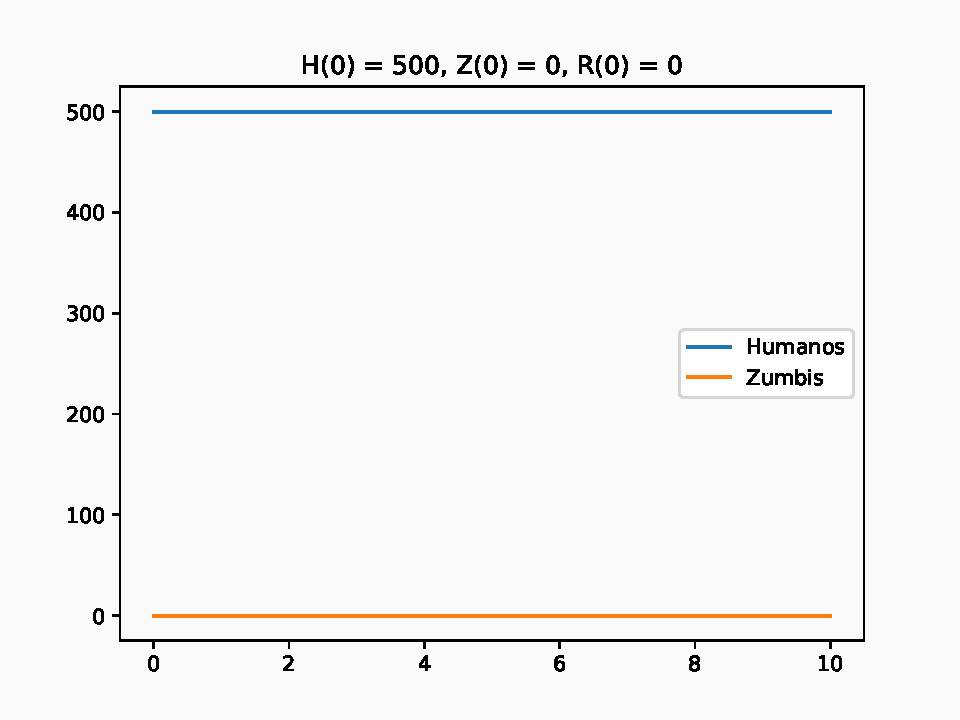
\includegraphics[width=0.75\textwidth]{1.pdf}
        \end{center}
    \end{frame}
    \begin{frame}
        \begin{center}
            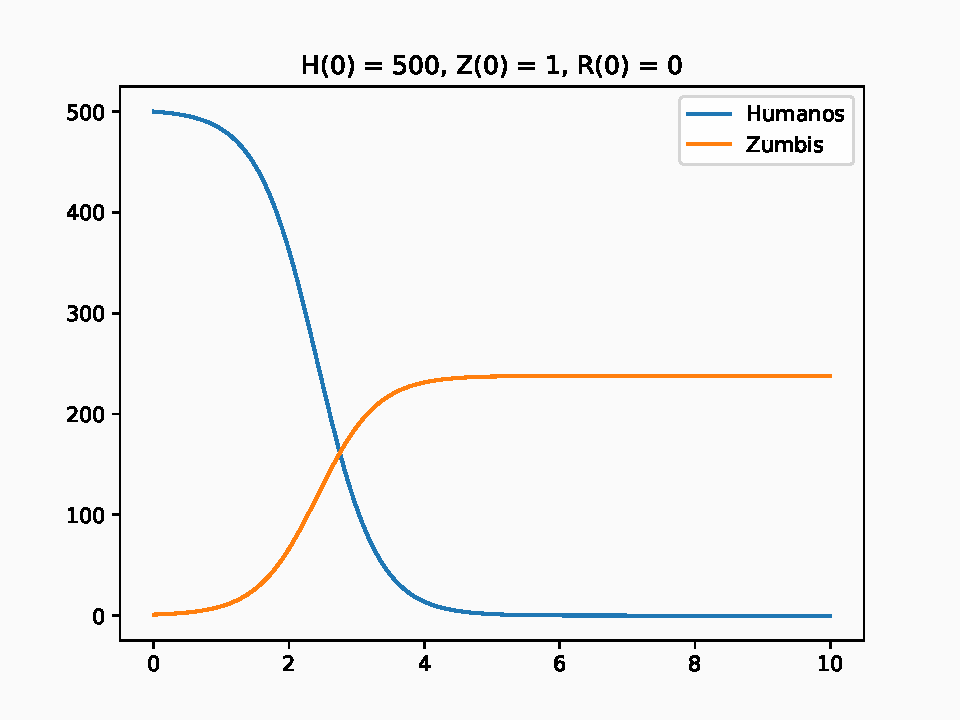
\includegraphics[width=0.75\textwidth]{2.pdf}
        \end{center}
    \end{frame}
    \begin{frame}
        \begin{center}
            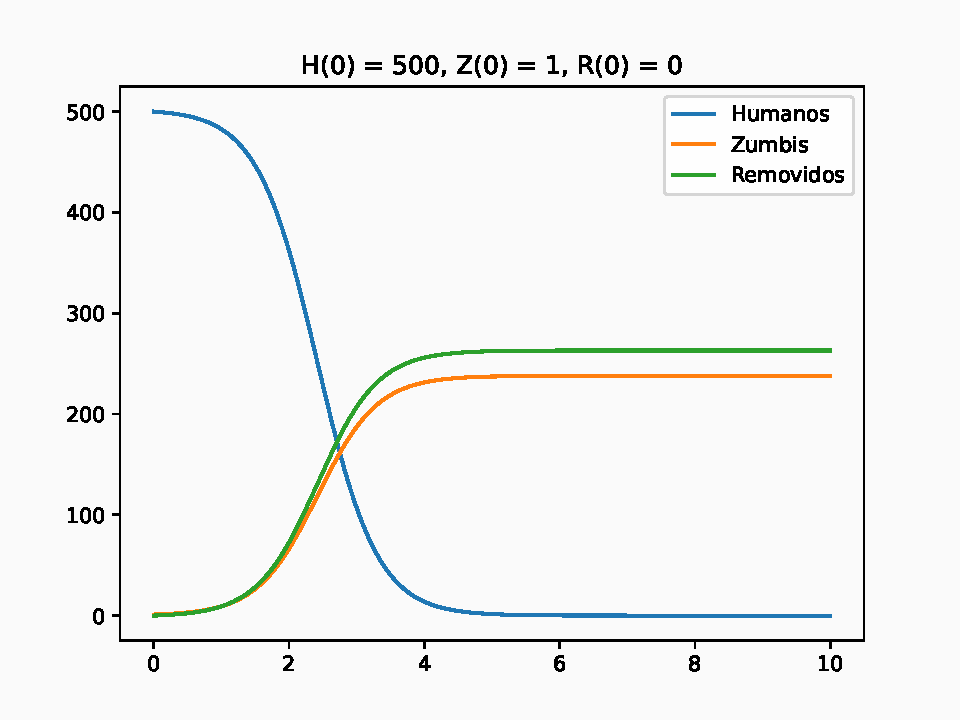
\includegraphics[width=0.75\textwidth]{3.pdf}
        \end{center}
    \end{frame}
    \begin{frame}
        \begin{center}
            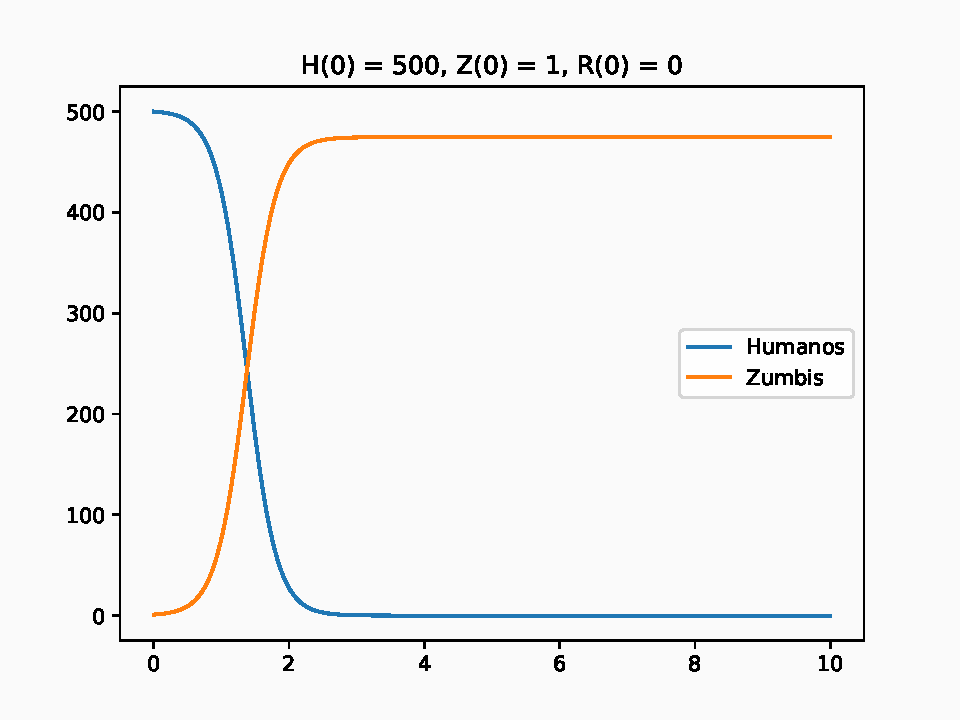
\includegraphics[width=0.75\textwidth]{4.pdf}
        \end{center}
    \end{frame}
    \begin{frame}
        \nocite{*}
        \printbibliography
    \end{frame}
\end{document}